\documentclass[letterpaper]{article}

\usepackage{natbib,alifeconf}
\usepackage{url,amsmath,amssymb}
\usepackage[colorlinks,allcolors=black]{hyperref}
\usepackage{booktabs}

\title{Supplementary Material:\\Conchordal: Emergent Harmony via Direct Cognitive Coupling\\in a Psychoacoustic Landscape}

\author{
    Koichi Takahashi$^{1,2}$
    \mbox{}\\
    $^1$Institute for Advanced Biosciences, Graduate School of Media and Governance, Keio University \\
    $^2$Conchordal.org \\
    info@conchordal.org
}

\renewcommand{\thetable}{S\arabic{table}}
\renewcommand{\thefigure}{S\arabic{figure}}
\renewcommand{\theequation}{S\arabic{equation}}

\begin{document}

\maketitle

\section{S1. Algorithm Pseudocode}

\subsection{S1.1 Pitch Adaptation (Experiment 1)}

\noindent\textbf{Input:} agents $\{a_1,\ldots,a_N\}$ with pitches $x_i$ in $\log_2$-freq space.\\
\textbf{Parameters:} step size $\lambda\!=\!15$\,ct, crowding weight $\lambda_C\!=\!0.15$, $T_0\!=\!0.05$, $\tau\!=\!30$.

\smallskip
\noindent\texttt{for} sweep $t = 0$ \texttt{to} $49$:\\
\hspace*{1em}$T_t \gets T_0 \cdot \exp(-t/\tau)$\\
\hspace*{1em}\texttt{for} each agent $a_i$:\\
\hspace*{2em}$\delta \sim \mathrm{Uniform}(-\lambda,\,+\lambda)$; \quad $x' \gets x_i + \delta$\\
\hspace*{2em}$P(x) = \lambda_C \sum_{j \neq i} K_{\text{crowd}}(\Delta_{\text{erb}}(x,x_j))$\\
\hspace*{2em}$S_{\text{old}} \gets s(t) \cdot C_{\text{field}}(x_i) - P(x_i)$\\
\hspace*{2em}$S_{\text{new}} \gets s(t) \cdot C_{\text{field}}(x') - P(x')$\\
\hspace*{2em}\texttt{if} $U(0,1) < \min\!\bigl(1,\,\exp\bigl((S_{\text{new}} - S_{\text{old}})/T_t\bigr)\bigr)$ \texttt{then} $x_i \gets x'$

\smallskip
\noindent where $s(t) = -1$ for $t \leq 24$ (dissonance-seeking), $+1$ for $t \geq 25$ (consonance-seeking).

\subsection{S1.2 Metabolic Policy (Experiment 2)}

\noindent\textbf{Parameters:} $c_b\!=\!0.5$/s, $c_a\!=\!0.02$, $r_E\!=\!0.5$, $\Delta t = 512/48000$\,s.

\smallskip
\noindent\texttt{for} each time step:\\
\hspace*{1em}\texttt{for} each agent $a_i$:\\
\hspace*{2em}$E_i \gets E_i - c_b \cdot \Delta t$ \hfill\textit{(basal drain)}\\
\hspace*{2em}\texttt{if} phase $\phi_i$ crosses zero \texttt{and} $E_i > 0$: \hfill\textit{(attack event)}\\
\hspace*{3em}$C_{\text{level01}} \gets \sigma\!\bigl(2 \cdot C_{\text{field}}(x_i)\bigr)$\\
\hspace*{3em}$E_i \gets E_i - c_a + r_E \cdot C_{\text{level01}}$\\
\hspace*{2em}\texttt{if} $E_i \leq 0$: agent dies; respawn at random pitch within $\pm 1$\,oct

\subsection{S1.3 Shared Rhythm Scaffold (Experiment 3)}

\noindent\textbf{Parameters:} $k_{\text{time}}\!=\!3.0$, kick at 2\,Hz, $\omega_0\!=\!1.8\!\cdot\!2\pi$\,rad/s, $\pm 2\%$ jitter.

\smallskip
\noindent\texttt{for} each time step $dt$:\\
\hspace*{1em}Advance canonical beat phase $\theta(t)$ at 2\,Hz\\
\hspace*{1em}\texttt{if} condition = scrambled \texttt{and} cycle boundary crossed: sample new offset $\psi \sim \mathrm{Uniform}(0,2\pi)$\\
\hspace*{1em}\texttt{for} each agent $a_i$:\\
\hspace*{2em}Set drive phase $\theta_i^{\ast} \gets \theta(t)$ (shared), $\theta(t)+\psi$ (scrambled), or none (off)\\
\hspace*{2em}$k_{\text{eff},i} \gets k_{\text{time}}$ (shared/scrambled) or $0$ (off)\\
\hspace*{2em}$\dot{\phi}_i \gets \omega_i + (k_{\text{eff},i}/N)\sum_j \sin(\phi_j - \phi_i) + F(\theta_i^{\ast})$\\
\hspace*{2em}$\phi_i \gets \phi_i + \dot{\phi}_i \cdot dt$\\
\hspace*{1em}Record PLV and onset phase relative to the canonical beat $\theta(t)$

\subsection{S1.4 Hereditary Respawn (Experiment 4)}

\noindent\textbf{Parameters:} mutation $\sigma\!=\!0.003\,\log_2$, crowding weight $\lambda_C$.

\smallskip
\noindent\texttt{for} each time step:\\
\hspace*{1em}Run metabolic policy (S1.2) with recharge enabled\\
\hspace*{1em}\texttt{if} agent $a_i$ dies ($E_i \leq 0$):\\
\hspace*{2em}Select parent $a_p$ uniformly from surviving agents\\
\hspace*{2em}$x_{\text{new}} \sim \mathcal{N}(x_p,\,\sigma^2)$; clamp to anchor $\pm 1$\,oct\\
\hspace*{2em}Respawn at $x_{\text{new}}$ with $E = 1.0$

\smallskip
\noindent\textbf{Random control:} respawn at $\mathrm{Uniform}(\text{anchor} \pm 1\,\text{oct})$ instead.

\section{S2. Normalization of $H_{01}$ and $R_{01}$}

Both harmonicity and roughness are normalized to $[0,1]$ before entering the consonance core.

\subsection{Harmonicity ($H_{01}$)}

The raw harmonicity potential from sibling projection (Eqs.~1--2 in the main text) is normalized by dividing by the self-harmonicity of a single harmonic tone at the reference position (which equals the kernel's maximum response):
\begin{equation}
H_{01}(x) = \mathrm{clamp}\!\left(\frac{H_{\mathrm{raw}}(x)}{H_{\mathrm{ref,max}}},\;0,\;1\right),
\end{equation}
where $H_{\mathrm{ref,max}} = 1.0$ (the kernel is pre-normalized so that a single harmonic stack produces unit peak).

\subsection{Roughness ($R_{01}$)}

Raw roughness is first expressed as a ratio $\rho = R_{\mathrm{raw}} / R_{\mathrm{ref}}$, where $R_{\mathrm{ref}}$ is the roughness of a single-tone reference density (computed once at initialization). This ratio is then mapped through a piecewise saturation function with physiological constant $k$ ($k\!=\!1.0$ in all experiments):
\begin{equation}
R_{01}(\rho) =
\begin{cases}
0 & \rho \leq 0,\\[2pt]
\displaystyle\frac{\rho}{1+k} & 0 < \rho < 1,\\[6pt]
\displaystyle 1 - \frac{k}{\rho + k} & \rho \geq 1,
\end{cases}
\end{equation}
clamped to $[0,1]$. For $\rho < 1$ (below-reference roughness) the mapping is linear; for $\rho \geq 1$ it is a hyperbolic saturation that approaches 1 asymptotically as $\rho \to \infty$. At $\rho = 1$ the function is continuous: $R_{01}(1) = 1/(1+k)$. With $k=1$, the reference roughness maps to $R_{01} = 0.5$.

\section{S3. Complete Parameter Table}

Table~S1 lists all parameters used across experiments.

\begin{table*}[t]
\centering
\caption{Complete parameter listing for all experiments.}
\label{tab:params}
\footnotesize
\begin{tabular}{@{}llcccc@{}}
\toprule
\textbf{Parameter} & \textbf{Symbol} & \textbf{Exp.\,1} & \textbf{Exp.\,2} & \textbf{Exp.\,3} & \textbf{Exp.\,4} \\
\midrule
Anchor frequency & $f_0$ & 220\,Hz & 220\,Hz & 220\,Hz & 220\,Hz \\
Population size & $N$ & 24 & 32 & 32 & 32 \\
Seeds & & 20 & 20 & 20 & 20 \\
Pitch range & & $\pm 2$\,oct & $\pm 1$\,oct & $\pm 1$\,oct & $\pm 1$\,oct \\
\midrule
\multicolumn{6}{@{}l}{\emph{Harmonicity / Roughness}} \\
Harmonic order & $N_H$ & 16 & 16 & 16 & 16 \\
Power-law exponent & $\rho$ & 0.4 & 0.4 & 0.4 & 0.4 \\
Roughness saturation & $k$ & 1.0 & 1.0 & 1.0 & 1.0 \\
\midrule
\multicolumn{6}{@{}l}{\emph{Consonance core}} \\
$C_{\text{field}}$ coefficients & $(a,b,c,d)$ & $(1,-1.35,1,0)$ & $(1,-1.35,1,0)$ & $(1,-1.35,1,0)$ & $(1,-1.35,1,0)$ \\
$C_{\text{density}}$ coefficients$^\ddagger$ & $(a,b,c,d)$ & $(1,0,-1,0)$ & --- & --- & --- \\
Sigmoid $(\beta,\theta)$ & & --- & $(2,0)$ & --- & $(2,0)$ \\
\midrule
\multicolumn{6}{@{}l}{\emph{Pitch adaptation}} \\
Step size & $\lambda$ & 0.15\,st & --- & --- & --- \\
Crowding weight & $\lambda_C$ & 0.15 & --- & --- & 0.15 \\
Initial temperature & $T_0$ & 0.05 & --- & --- & --- \\
Annealing time constant & $\tau$ & 30 steps & --- & --- & --- \\
Duration & & 50 sweeps & --- & --- & --- \\
Phase switch & & step 25 & --- & --- & --- \\
Burn-in discarded & & 10 steps & --- & --- & --- \\
\midrule
\multicolumn{6}{@{}l}{\emph{Metabolism}} \\
Basal cost & $c_b$ & --- & 0.5/s & --- & 0.5/s \\
Attack cost & $c_a$ & --- & 0.02 & --- & 0.02 \\
Recharge coefficient & $r_E$ & --- & 0.5/att & --- & 0.5/att \\
Energy cap & $E_{\text{cap}}$ & --- & 1.0 & --- & 1.0 \\
Time step & $\Delta t$ & --- & 512/48k\,s & 0.02\,s & 512/48k\,s \\
Termination & & --- & 200 deaths & 40\,s & 4000 deaths \\
\midrule
\multicolumn{6}{@{}l}{\emph{Temporal coupling}} \\
Base coupling & $k_{\text{time}}$ & --- & --- & 3.0 & --- \\
External kick & $f_{\text{kick}}$ & --- & --- & 2\,Hz & --- \\
Intrinsic frequency & $\omega_0$ & --- & --- & $1.8 \cdot 2\pi$ & --- \\
Frequency jitter & & --- & --- & $\pm 2\%$ & --- \\
\midrule
\multicolumn{6}{@{}l}{\emph{Heredity}} \\
Mutation $\sigma$ & $\sigma_m$ & --- & --- & --- & $0.003\,\log_2$ \\
Parent selection & & --- & --- & --- & uniform \\
\midrule
\multicolumn{6}{@{}l}{\emph{JI cross-validation}} \\
Proximity kernel & $\alpha$ & --- & --- & --- & $4.0 \times 10^{-4}\,\text{ct}^{-2}$ \\
Ratio limit & $p,q$ & --- & --- & --- & $\leq 8$ \\
Ratio weight & & --- & --- & --- & $1/(pq)$ \\
\bottomrule
\multicolumn{6}{@{}l}{\footnotesize $^\ddagger$ Visualization only (Figure~1D); not used in experiment algorithms.}
\end{tabular}
\end{table*}

\subsection{S3.1 Supplementary Mechanism Check: Configurable Spectral--Temporal Bridge}

The relation between Conchordal's spectral and temporal axes is not treated as a uniquely determined neurocognitive law. Existing neuroscience motivates several plausible couplings between harmonic structure, salience, attention, and rhythmic prediction, but does not reduce them to a single fixed mapping. Conchordal therefore treats the bridge from spectral state to temporal coupling as a design degree of freedom available to the composer. The current implementation includes one such mapping: consonance modulates metabolic vitality, and vitality gates the effective coupling strength of the phase oscillator. In the supplementary assay shown here, the bridge uses $R=1.0$/s, $\gamma=0.5$/s, $E_{\text{cap}}=1.0$, $\lambda_v=1.0$, and $v_{\text{floor}}=0.0$. Figure~\ref{fig:supp-e5-bridge} reports this assay as an implementation-level mechanism check, not as evidence that consonance uniquely determines rhythmic coupling in biological cognition.

\begin{figure*}[t]
\centering
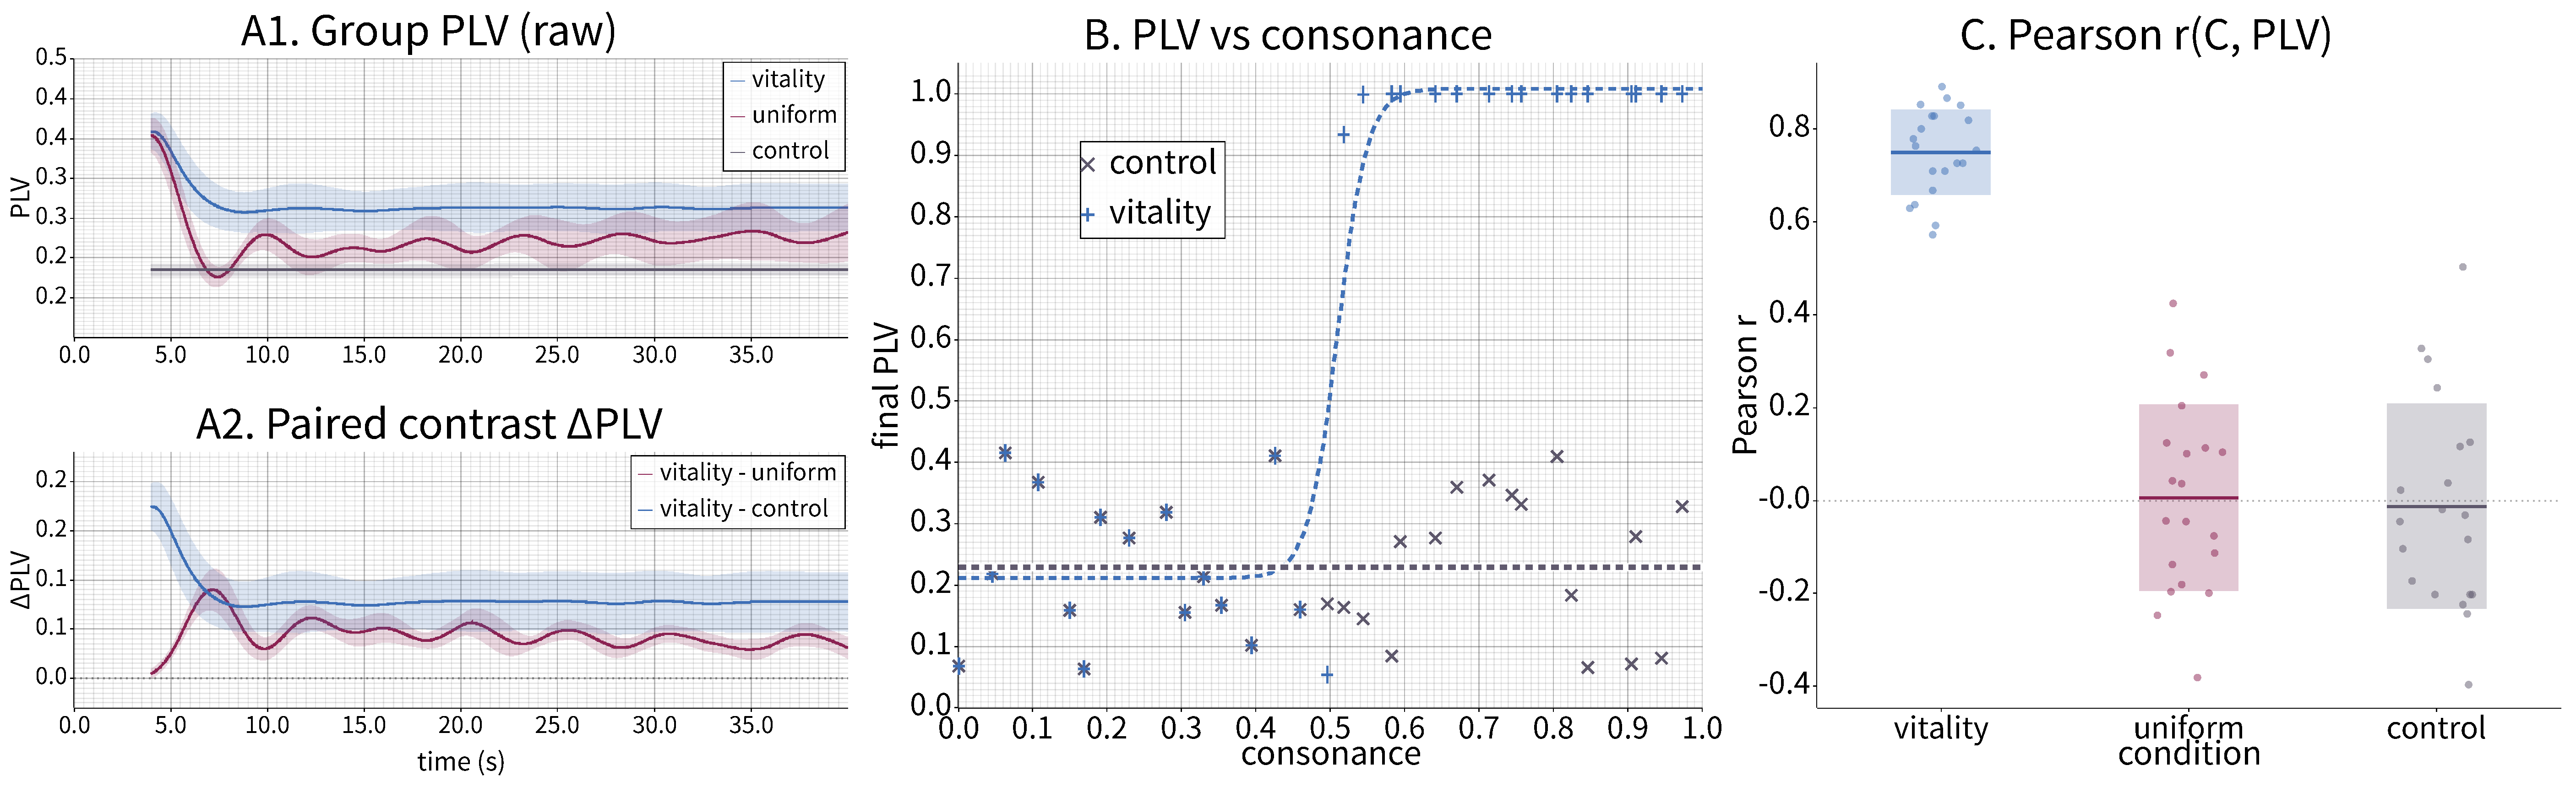
\includegraphics[width=\textwidth]{experiments/plots/e5/paper_e5_figure.pdf}
\caption{Supplementary mechanism check for one configurable spectral--temporal bridge (20 seeds $\times$ 3 conditions). (A1)~Group mean PLV over time (95\% CI). (A2)~Paired contrast $\Delta$PLV (95\% CI). (B)~Per-agent final PLV vs.\ $C_{\text{field}}$ (representative seed) with sigmoid fit ($c_{50}$ fixed at 0). (C)~Seed-level Pearson $r(C_{\text{field}},\,\text{PLV})$. In the current implementation, vitality-gated coupling yields a graded bridge from spectral state to entrainment strength; alternative bridge mappings remain possible within the broader Conchordal design.}
\label{fig:supp-e5-bridge}
\end{figure*}

\section{S4. Experiment 4: Full Sweep Results}

Table~S2 reports the hereditary adaptation parameter sweep. Each of the 15 conditions was run with 20 seeds per arm (heredity vs.\ random control). The reported setting in the main text ($\sigma\!=\!0.003$, deaths $=\!4{,}000$, $N\!=\!32$) is marked with $\star$.

\begin{table*}[t]
\centering
\caption{Full parameter sweep for Experiment~4 (hereditary adaptation). Each row reports one parameter setting; ``Sep.''\ is the mean $\Delta C_{\text{score}}$(heredity) $-$ mean $\Delta C_{\text{score}}$(random). Welch's $t$-test compares the two arms ($n\!=\!20$ seeds each). $\star$ marks the setting reported in the main text.}
\label{tab:sweep}
\footnotesize
\begin{tabular}{@{}rrrccccc@{}}
\toprule
$\sigma$ & Deaths & $N$ & $\overline{\Delta C}_{\text{her}}$ & $\overline{\Delta C}_{\text{rnd}}$ & Sep. & $t$ & $p$ \\
\midrule
0.001 & 2000 & 32 & $0.074 \pm 0.150$ & $0.004 \pm 0.035$ & 0.071 & 2.06 & 0.052 \\
0.001 & 3000 & 32 & $0.117 \pm 0.174$ & $0.007 \pm 0.025$ & 0.111 & 2.81 & 0.011$^*$ \\
0.002 & 2000 & 32 & $0.067 \pm 0.119$ & $0.004 \pm 0.035$ & 0.063 & 2.29 & 0.032$^*$ \\
0.002 & 3000 & 32 & $0.039 \pm 0.093$ & $0.007 \pm 0.025$ & 0.032 & 1.49 & 0.151 \\
0.003 & 2000 & 16 & $0.035 \pm 0.101$ & $-0.004 \pm 0.036$ & 0.039 & 1.62 & 0.118 \\
0.003 & 2000 & 24 & $0.089 \pm 0.155$ & $0.004 \pm 0.029$ & 0.085 & 2.41 & 0.025$^*$ \\
0.003 & 2000 & 32 & $0.096 \pm 0.138$ & $0.004 \pm 0.035$ & 0.093 & 2.91 & 0.008$^*$ \\
0.003 & 2000 & 48 & $0.061 \pm 0.141$ & $0.004 \pm 0.021$ & 0.058 & 1.80 & 0.087 \\
0.003 & 3000 & 32 & $0.118 \pm 0.160$ & $0.007 \pm 0.025$ & 0.111 & 3.07 & 0.006$^*$ \\
$\star$\,0.003 & 4000 & 32 & $0.121 \pm 0.177$ & $-0.003 \pm 0.027$ & 0.124 & 3.10 & 0.006$^*$ \\
0.003 & 5000 & 32 & $0.113 \pm 0.167$ & $-0.003 \pm 0.025$ & 0.116 & 3.07 & 0.006$^*$ \\
0.005 & 2000 & 32 & $0.078 \pm 0.135$ & $0.004 \pm 0.035$ & 0.075 & 2.40 & 0.026$^*$ \\
0.005 & 3000 & 32 & $0.072 \pm 0.119$ & $0.007 \pm 0.025$ & 0.065 & 2.39 & 0.027$^*$ \\
0.01 & 2000 & 32 & $0.058 \pm 0.102$ & $0.004 \pm 0.035$ & 0.054 & 2.25 & 0.034$^*$ \\
0.02 & 2000 & 32 & $0.106 \pm 0.135$ & $0.004 \pm 0.035$ & 0.102 & 3.26 & 0.004$^*$ \\
\bottomrule
\multicolumn{8}{@{}l}{\footnotesize $^*$Significant at $p < 0.05$. $\star$ = reported setting in the main text ($\sigma\!=\!0.003$, 4{,}000 deaths, $N\!=\!32$).}
\end{tabular}
\end{table*}

\section{S5. Bilinear Consonance Core: Derivation}

The consonance core (Eq.~5 in the main text) is the most general bilinear form for two inputs $H_{01}, R_{01} \in [0,1]$:
\begin{equation}
C = a\,H_{01} + b\,R_{01} + c\,H_{01}\,R_{01} + d.
\end{equation}

\noindent\textbf{$C_{\text{field}}$} $(a,b,c,d) = (1, -1.35, 1, 0)$:
\begin{align}
C_{\text{field}} &= H_{01} - 1.35\,R_{01} + H_{01}\,R_{01} \\
                 &= H_{01}(1 + R_{01}) - 1.35\,R_{01}.
\end{align}
When $H_{01}$ is high (strong harmonicity), the $H_{01}\,R_{01}$ term partially compensates for roughness, reflecting the perceptual observation that harmonically rich intervals tolerate moderate beating. When $H_{01} = 0$, roughness is penalized at full strength.

\noindent\textbf{$C_{\text{density}}$} $(a,b,c,d) = (1, 0, -1, 0)$:
\begin{equation}
C_{\text{density}} = H_{01}(1 - R_{01}).
\end{equation}
This product is nonnegative and peaks where harmonicity is high and roughness is low. In Conchordal's interactive mode it serves as a spawn-position weight; it is not used in the experiments reported in this paper but is shown in Figure~1D for comparison.

\noindent\textbf{$C_{\text{level01}}$}: $C_{\text{field}}$ passed through a logistic sigmoid $\sigma(\beta(x - \theta))$ with $\beta=2$, $\theta=0$. This bounds the metabolic signal to $[0,1]$ while preserving the ranking.

\section{S6. Sign-Flip Permutation Test}

The interaction contrast for the integration test (Figure~7 in the main text) is tested with a one-sample sign-flip permutation test:

\begin{enumerate}
\item For each of $n=20$ matched seeds, compute the contrast $d_i = \text{HH}_i - \text{H}_i - \text{RH}_i + \text{R}_i$.
\item Under $H_0$: $E[d_i] = 0$, each $d_i$ is equally likely to be positive or negative. For each of $2^{20} = 1{,}048{,}576$ sign patterns $s \in \{-1,+1\}^{20}$, compute $\bar{d}_s = \frac{1}{n}\sum_i s_i \, d_i$.
\item The $p$-value is the fraction of sign patterns yielding $|\bar{d}_s| \geq |\bar{d}_{\text{obs}}|$.
\end{enumerate}

Because $n=20$, exact enumeration is feasible. The observed $p = 0.000053$ (1 in 18{,}868 patterns) with mean contrast $0.30$ (95\% CI $[0.20, 0.39]$).

\section{S7. Consonance-Only Control (Experiment 1)}

Experiment~1 uses a two-phase curriculum: dissonance-seeking (steps 0--24) followed by consonance-seeking (steps 25--49). To assess whether the resulting polyphony depends on this schedule, we ran a \emph{consonance-only} control with identical parameters but $s(t) = +1$ for all 50 sweeps (\emph{local-search} condition, 20 seeds).

\begin{table}[h]
\centering
\caption{Curriculum vs.\ consonance-only control (Experiment~1, \emph{local-search} condition, $n\!=\!20$ seeds).}
\label{tab:consonly}
\footnotesize
\begin{tabular}{@{}lccc@{}}
\toprule
\textbf{Metric} & \textbf{Curriculum} & \textbf{Cons.-only} & $t$ \\
\midrule
$C_{\text{score}}$ (post) & $0.731 \pm 0.057$ & $0.731 \pm 0.041$ & $-0.02$ \\
Unique pitch bins & $9.4 \pm 1.2$ & $5.9 \pm 0.6$ & $-11.6^{***}$ \\
NN distance (st) & $0.324 \pm 0.245$ & $0.049 \pm 0.068$ & $-4.8^{***}$ \\
Interval entropy & $1.52 \pm 0.36$ & $1.65 \pm 0.27$ & $1.4$ \\
\bottomrule
\end{tabular}
\end{table}

Both conditions reach indistinguishable final consonance ($C_{\text{score}} = 0.731$; $p = 0.98$), confirming that consonant structure emerges from the landscape--penalty interaction regardless of schedule. However, the curriculum significantly improves pitch diversity: more unique bins ($9.4$ vs.\ $5.9$; $p < 0.0001$) and wider nearest-neighbour spacing ($0.324$ vs.\ $0.049$\,st; $p = 0.0001$), while interval entropy does not differ significantly ($p = 0.19$). The dissonance-seeking phase thus serves as an initialisation strategy that broadens the pitch distribution, preventing premature collapse to a small number of positions.

\section{S7.1 Derived Metrics: LOO Score and Scene Consonance}

\noindent\textbf{Leave-One-Out (LOO) Score.}
For each agent~$i$, the field spectrum is recomputed with agent~$i$'s harmonic contribution removed, yielding a leave-one-out field $F_{-i}$.
The agent's LOO consonance is the consonance field evaluated at its own position~$x_i$ against the remaining agents:
\begin{equation}
C_{\text{score},i} = C_{\text{field}}(F_{-i},\, x_i).
\end{equation}
The population mean defines the primary outcome metric:
\begin{equation}
C_{\text{score}} = \frac{1}{N}\sum_{i=1}^{N} C_{\text{score},i}.
\end{equation}

\noindent\textbf{Scene Consonance $G(F)$.}
Scene harmonicity $H_{\text{soc}}$ and roughness $R_{\text{soc}}$ quantify the \emph{emergent} harmonic and roughness structure beyond what individual agents would produce in isolation.
Let $H(F)$ and $R(F)$ denote harmonicity and roughness evaluated on the full scene spectrum~$F$, and let $H(\{i\})$ and $R(\{i\})$ denote the same quantities for agent~$i$ presented alone.
Then:
\begin{align}
H_{\text{soc}} &= H(F) - \frac{1}{N}\sum_{i=1}^{N} H(\{i\}),\\
R_{\text{soc}} &= R(F) - \frac{1}{N}\sum_{i=1}^{N} R(\{i\}).
\end{align}
Scene consonance applies the same bilinear core (Eq.~5 in the main text):
\begin{equation}
G(F) = a\,H_{\text{soc}} + b\,R_{\text{soc}} + c\,H_{\text{soc}}\,R_{\text{soc}}.
\end{equation}
By subtracting the mean singleton contribution, $G(F)$ isolates the consonance arising from inter-agent spectral interactions rather than individual tonal quality.

\section{S8. Terrain Control and Robustness Analysis}

Three supplementary analyses test whether the self-organised polyphony reported in Experiment~1 depends on the specific structure of the psychoacoustic landscape rather than on incidental parameter choices.

\subsection{S8.1 Shuffled-Landscape Control}

We destroy spatial coherence by applying a fixed random permutation of the $C_{\text{score}}$ bin indices, generated once per run and held fixed throughout all sweeps.
Agents therefore move on a stationary landscape with the same \emph{marginal} score distribution but no local gradient structure.
Table~\ref{tab:shuffled} compares the shuffled condition with the standard \emph{local-search} condition ($n=20$ seeds each).

\begin{table}[h]
\centering
\caption{\emph{Local-search} vs.\ shuffled landscape (Experiment~1).}
\label{tab:shuffled}
\footnotesize
\begin{tabular}{@{}lccr@{}}
\toprule
\textbf{Metric} & \textbf{Local-search} & \textbf{Shuffled} & $t$ \\
\midrule
Unique pitch bins & $9.4 \pm 1.2$ & $9.6 \pm 1.0$ & $0.6$ \\
NN distance (st)  & $0.324 \pm 0.245$ & $0.328 \pm 0.207$ & $0.1$ \\
Interval entropy  & $1.52 \pm 0.36$ & $3.36 \pm 0.27$ & $18.6^{***}$ \\
$C_{\text{score}}$ (ref) & $0.731 \pm 0.057$ & $0.459 \pm 0.042$ & $-17.3^{***}$ \\
\bottomrule
\end{tabular}
\end{table}

$C_{\text{score}}$ (ref) denotes the consonance score of each final configuration evaluated on the \emph{original} (unshuffled) landscape, enabling a fair cross-condition comparison.
Without coherent spatial gradients, agents still spread across the register (similar unique-bin count and nearest-neighbour spacing) thanks to the crowding penalty, but the interval structure degrades sharply: entropy rises from $1.52$ to $3.36$\,nats ($p < 0.0001$), and $C_{\text{score}}$ drops from $0.731$ to $0.459$ ($p < 0.0001$).
The coherent psychoacoustic landscape is therefore necessary for agents to self-organise into musically structured pitch configurations.

\subsection{S8.2 Harmonicity--Roughness Misalignment Control}

The consonance kernel combines harmonicity ($H_{01}$) and roughness ($R_{01}$).
We test whether their spatial alignment matters by circularly shifting $R_{01}$ by $\Delta$ cents before scoring, which preserves each component's marginal statistics but breaks the psychoacoustically motivated registration between them.
Four shift values span the range $\Delta \in \{137, 271, 389, 523\}$\,cents.
Table~\ref{tab:misaligned} reports the results ($n=20$ seeds per shift, 80 runs total for the misaligned aggregate).

\begin{table}[h]
\centering
\caption{\emph{Local-search} vs.\ H/R-misaligned conditions (Experiment~1).}
\label{tab:misaligned}
\footnotesize
\begin{tabular}{@{}lccc@{}}
\toprule
Condition & Unique bins & NN dist.\ (st) & Entropy \\
\midrule
Local-search        & $9.4 \pm 1.2$ & $0.324 \pm 0.245$ & $1.52 \pm 0.36$ \\
$\Delta = 137$\,¢   & $5.9 \pm 1.0$ & $0.047 \pm 0.081$ & $1.72 \pm 0.30$ \\
$\Delta = 271$\,¢   & $6.4 \pm 0.8$ & $0.062 \pm 0.078$ & $1.83 \pm 0.29$ \\
$\Delta = 389$\,¢   & $6.2 \pm 1.0$ & $0.065 \pm 0.103$ & $1.74 \pm 0.27$ \\
$\Delta = 523$\,¢   & $5.8 \pm 0.9$ & $0.032 \pm 0.054$ & $1.57 \pm 0.31$ \\
\midrule
Misaligned (avg)    & $6.1 \pm 1.0$ & $0.052 \pm 0.082$ & $1.72 \pm 0.31$ \\
\bottomrule
\end{tabular}
\end{table}

All four misaligned conditions produce significantly fewer unique pitch bins than the local-search baseline (all $p < 10^{-4}$, Welch $t$), dropping from $9.4$ to $\approx$6 bins---comparable to the consonance-only control (S7).
Nearest-neighbour distances also decrease significantly (all $p \le 0.0002$).
Entropy effects are mixed: two shifts reach $p < 0.05$ while two do not, and the aggregate is significant ($p = 0.0002$).
Misalignment thus preserves consonance (all $C_{\text{score}} \ge 0.70$) but eliminates the diversity benefit of the curriculum, reinforcing the conclusion from the shuffled-landscape control (S8.1) that a coherent landscape gradient is essential for structured polyphony.

\subsection{S8.3 Consonance Kernel Coefficient Sensitivity}

The consonance kernel $C = a\,H_{01} + b\,R_{01} + c\,H_{01}\,R_{01} + d$ has four coefficients; the default is $(a,b,c,d) = (1.0, {-}1.35, 1.0, 0.0)$.
We sweep $b \in \{-2.0, {-}1.35, {-}0.7, 0.0\}$ and $c \in \{0.0, 0.5, 1.0, 1.5\}$ with $a=1$, $d=0$ fixed (16 conditions, 20 seeds each).
Table~\ref{tab:coeff} reports the results; because the sweep varies the kernel while holding everything else constant, it isolates the sensitivity of the consonance landscape to its parameterisation.

\begin{table}[h]
\centering
\caption{Coefficient sweep: polyphony metrics across 16 $(b,c)$ settings.}
\label{tab:coeff}
\footnotesize
\begin{tabular}{@{}rrccc@{}}
\toprule
$b$ & $c$ & Unique bins & Entropy & $C_{\text{score}}$ \\
\midrule
$-2.00$ & $0.00$ & $6.2 \pm 1.0$ & $1.65 \pm 0.26$ & $0.738 \pm 0.053$ \\
$-2.00$ & $0.50$ & $5.8 \pm 1.1$ & $1.61 \pm 0.33$ & $0.729 \pm 0.051$ \\
$-2.00$ & $1.00$ & $6.2 \pm 1.1$ & $1.63 \pm 0.26$ & $0.746 \pm 0.043$ \\
$-2.00$ & $1.50$ & $6.1 \pm 1.2$ & $1.67 \pm 0.29$ & $0.751 \pm 0.042$ \\
$-1.35$ & $0.00$ & $6.2 \pm 1.2$ & $1.66 \pm 0.28$ & $0.736 \pm 0.047$ \\
$-1.35$ & $0.50$ & $6.2 \pm 1.0$ & $1.67 \pm 0.32$ & $0.733 \pm 0.048$ \\
$-1.35$ & $1.00$ & $6.4 \pm 0.7$ & $1.84 \pm 0.29$ & $0.734 \pm 0.035$ \\
$-1.35$ & $1.50$ & $5.9 \pm 1.1$ & $1.61 \pm 0.33$ & $0.760 \pm 0.043$ \\
$-0.70$ & $0.00$ & $6.5 \pm 1.0$ & $1.74 \pm 0.28$ & $0.739 \pm 0.042$ \\
$-0.70$ & $0.50$ & $6.1 \pm 1.0$ & $1.71 \pm 0.31$ & $0.761 \pm 0.034$ \\
$-0.70$ & $1.00$ & $5.8 \pm 1.2$ & $1.61 \pm 0.33$ & $0.768 \pm 0.040$ \\
$-0.70$ & $1.50$ & $6.2 \pm 0.8$ & $1.66 \pm 0.22$ & $0.788 \pm 0.041$ \\
$0.00$  & $0.00$ & $6.3 \pm 1.2$ & $1.68 \pm 0.31$ & $0.763 \pm 0.034$ \\
$0.00$  & $0.50$ & $5.9 \pm 1.1$ & $1.75 \pm 0.28$ & $0.760 \pm 0.042$ \\
$0.00$  & $1.00$ & $6.2 \pm 0.8$ & $1.79 \pm 0.27$ & $0.792 \pm 0.034$ \\
$0.00$  & $1.50$ & $5.8 \pm 0.9$ & $1.71 \pm 0.23$ & $0.814 \pm 0.028$ \\
\bottomrule
\end{tabular}
\end{table}

Unique-bin counts ($5.8$--$6.5$) and entropy ($1.61$--$1.84$\,nats) are stable across the entire $(b,c)$ grid, showing that the emergent pitch structure is not fragile to kernel parameterisation.
$C_{\text{score}}$ increases when the roughness penalty $|b|$ decreases or the interaction weight $c$ increases ($0.729$--$0.814$), which is expected from the kernel definition.
The overall level of unique bins ($\approx$6) matches the consonance-only control (S7), confirming that the crowding penalty---not the kernel coefficients---is the primary driver of the higher diversity ($9.4$ bins) seen in the full local-search condition.

\subsection{S8.4 Integration Test Terrain Control (Experiment~4)}

To test whether the synergistic heredity$\times$hill-climbing interaction (main text, \S5.1) depends on the coherent structure of the psychoacoustic landscape, we repeated all four integration-test conditions on a shuffled landscape, yielding a complete $2 \times 2 \times 2$ factorial (heredity/random $\times$ hill-climbing on/off $\times$ real/shuffled terrain; 8 conditions $\times$ 20 seeds $= 160$ runs).

\begin{table}[h]
\centering
\caption{Full $2{\times}2{\times}2$ integration terrain control (20 seeds each).}
\label{tab:s7-integration-terrain}
\footnotesize
\begin{tabular}{@{}lccc@{}}
\toprule
Condition & Real & Shuffled & Diff. \\
\midrule
H  (her., no hill)  & $.185 \pm .076$ & $.051 \pm .006$ & $.134^{***}$ \\
HH (her.\ + hill)   & $.530 \pm .068$ & $.082 \pm .049$ & $.449^{***}$ \\
R  (rnd., no hill)   & $.061 \pm .008$ & $.059 \pm .008$ & $.003$ \\
RH (rnd.\ + hill)    & $.107 \pm .013$ & $.056 \pm .006$ & $.051^{***}$ \\
\midrule
\multicolumn{4}{@{}l}{Interaction contrast (real): $0.30$ [$0.20$, $0.39$], $p < 0.001$} \\
\multicolumn{4}{@{}l}{Interaction contrast (shuffled): $0.03$ [$-0.02$, $0.08$], $p = 0.19$} \\
\bottomrule
\end{tabular}
\end{table}

On real terrain, the interaction contrast is large and significant ($0.30$, $p < 0.001$); on the shuffled landscape the contrast drops to $0.03$ ($p = 0.19$), eliminating the synergy entirely.
The full factorial also reveals that coherent terrain affects the non-hill conditions asymmetrically: heredity benefits substantially from real terrain even without hill-climbing (H~real $0.185$ vs.\ H~shuffled $0.051$, $p = 0.0002$), because consonance-gated metabolism rewards agents that happen to inherit consonant positions, an effect that vanishes when the landscape is spatially incoherent.
Random respawn shows no such terrain dependence (R~real $0.061$ vs.\ R~shuffled $0.059$, $p = 0.70$), confirming that the metabolism-mediated terrain effect operates specifically through heritable pitch structure.

\subsection{S8.5 Topology Generalization (Experiment~4)}

To test whether the heredity$\times$hill-climbing interaction depends on the specific harmonicity profile used in the default configuration, we repeated the four real-terrain conditions (H, HH, R, RH; 20 seeds each) under three landscape topologies, generated by varying the number of environment partials in the anchor harmonic series (3, 6, 10). Fewer partials produce a smoother, broader harmonicity landscape; more partials increase spectral fine structure.

\begin{table}[h]
\centering
\caption{Topology generalization: interaction contrast across different numbers of environment partials (20 seeds each).}
\label{tab:s7-topology}
\footnotesize
\begin{tabular}{@{}lccccc@{}}
\toprule
Partials & H & HH & R & RH & Contrast [95\% CI] \\
\midrule
3  & .152 & .563 & .074 & .116 & $.37$ [.29,\,.45]$^{***}$ \\
6 (default)  & .185 & .530 & .061 & .107 & $.30$ [.21,\,.39]$^{***}$ \\
10 & .125 & .528 & .064 & .108 & $.36$ [.28,\,.44]$^{***}$ \\
\bottomrule
\multicolumn{6}{@{}l}{\footnotesize $^{***}p < 0.001$.}
\end{tabular}
\end{table}

The interaction contrast is large and significant ($p < 0.001$) across all three topologies, ranging from $0.30$ to $0.37$, confirming that the synergistic effect is not specific to the default harmonicity profile but generalizes across qualitatively different landscape structures.

\subsection{S8.6 Phase Coherence (Experiment~4)}

Each Experiment~4 agent entrains to a shared theta oscillator via a Kuramoto coupling mechanism. We computed the population Kuramoto order parameter $R = \lvert N^{-1} \sum_j e^{i(\phi_j - \phi_\theta)} \rvert$ at the final snapshot, where $\phi_j$ is each agent's rhythm phase and $\phi_\theta$ is the global theta phase ($R = 1$ indicates perfect synchrony; $R \approx 0$ indicates incoherence).

\begin{table}[h]
\centering
\caption{Phase coherence $R$ (Kuramoto order parameter) at the final snapshot (20 seeds each).}
\label{tab:s7-phase}
\footnotesize
\begin{tabular}{@{}lcc@{}}
\toprule
Condition & Real terrain & Shuffled \\
\midrule
H  (heredity, no hill)  & $0.183 \pm 0.027$ & $0.117 \pm 0.027$ \\
HH (heredity + hill)    & $0.163 \pm 0.036$ & $0.125 \pm 0.033$ \\
R  (random, no hill)    & $0.169 \pm 0.032$ & $0.165 \pm 0.029$ \\
RH (random + hill)      & $0.183 \pm 0.041$ & $0.181 \pm 0.039$ \\
\midrule
\multicolumn{3}{@{}l}{HH $-$ RH: $-0.020$ [$-0.078$, $0.039$], $p = 0.53$} \\
\multicolumn{3}{@{}l}{H $-$ R: $0.014$ [$-0.022$, $0.051$], $p = 0.47$} \\
\bottomrule
\end{tabular}
\end{table}

Phase coherence is low across all conditions ($R \approx 0.12\text{--}0.18$) and does not differ significantly between heredity and random conditions ($p > 0.4$). This indicates that in the current Experiment~4 parameterization, consonance-gated entrainment does not produce differential temporal binding across conditions within 4{,}000 deaths. On real terrain, heredity-type conditions show slightly higher $R$ than their shuffled counterparts (e.g., H: $0.183$ vs.\ $0.117$), consistent with the consonance-gated metabolic advantage providing agents more stable positions from which to entrain; random conditions show no such terrain dependence (R: $0.169$ vs.\ $0.165$).

\end{document}
